% !TEX encoding = UTF-8 Unicode
%!TEX root = thesis.tex
% !TEX spellcheck = en-US
\chapter[Result and Discussion]{Result and Discussion}
In this chapter the results of the experiments described in earlier chapters are presented discussed.
The chapter is divided into three sections, covering the 3 different types experiments that were run.
First the experimental optimization towards our systems properties are presented.
Then the experiment results regarding system performance will be presented.
Finally the results regarding the systems energy efficiency are presented.
The performance trade off from running energy efficient is also asserted here.

\section{Optimization}
Different systems may perform better with different programs.
To ensure that the results we find are represented by programs well suited for the system, the experiments were tested with different degrees of loop unrolling.
By unrolling loop iterations, the task sizes increase.
This reduce the overhead of initiating iterations.
It also reduce overhead related to loop control, like end of loop tests and loading data into new memory locations necessary for each loop iteration.
There is however a limit to how much unrolling can be done.
At some point the size of the task will create difficulties like early cache eviction of data.
The optimal amount of loop unrolling may vary from system to system.
Because of this, experiments were run on all the processor configurations that will be used for later experiments, with different unroll degrees.

\begin{figure}[H]
  \centering
  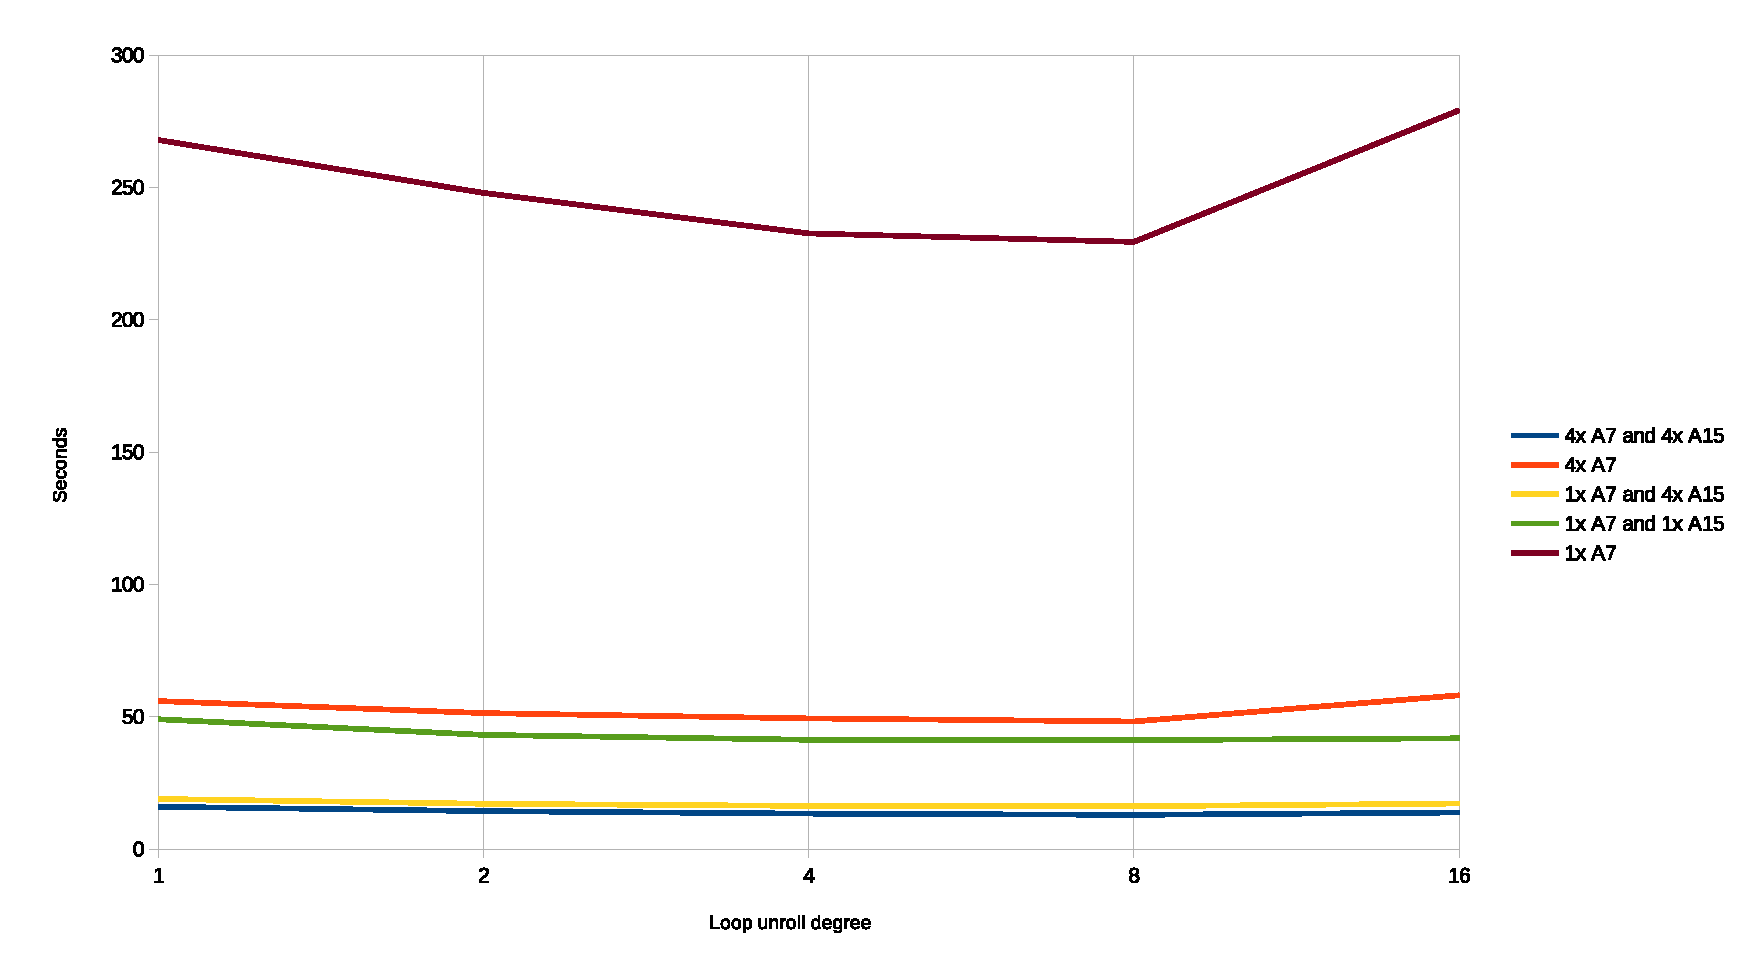
\includegraphics[width=160mm]{fig/loop-unroll-execution-time.eps}
  \caption{Execution time of 2D-Convolution with different degrees of loop unrolling running on different processor configurations. \label{overflow}}
\end{figure}
\begin{table}[H]
  \begin{tabular}{llllll}
    \toprule
    Processor configuration           & \multicolumn{5}{c}{Loop unroll degree} \\
                                      & 1                   & 2         & 4         & 8         & 16 \\
    \midrule
    4x Cortex-A7 and 4x Cortex-A15    & 15.9875             & 14.3006   & 13.3692   & 12.8891   & 13.8013 \\
    4x Cortex-A7                      & 55.8885             & 51.3407   & 49.3267   & 48.1665   & 58.0834 \\
    1x Cortex-A7 and 4x Cortex-A15    & 18.9248             & 17.082    & 16.279    & 16.1658   & 17.1759 \\
    1x Cortex-A7 and 1x Cortex-A15    & 49.0195             & 43.1061   & 41.2549   & 41.1286   & 41.8136 \\
    1x Cortex-A7                      & 267.8882            & 247.8783  & 232.5777  & 229.3884  & 279.1135 \\
    \bottomrule
  \end{tabular}
  \caption{Execution time of 2D-Convolution with different degrees of loop unrolling on different processor configurations. \label{overflow}}
\end{table}

The results show that a loop unroll degree of 8 was optimal for this specific implementation of 2D-Convolution on ODROID-XU3.
This was observed across the results with all tested processor configurations.
Because of this result, the remaining experiments are all run with a loop unroll degree of 8.

As mentioned loop unrolling is limited.
In 2D-Convolution there are many read write operations in the loop body.
As the size of this loop body increase, the amount of data accessed by each iteration grow.
Eventually this data does no longer fit in cache.
There is reason to suspect that this is what we are observing in the performance loss at loop unroll degree 16.

\section{Performance}
Even with energy efficiency as the focus, performance data are still interesting.
The data are both useful on their own to observe the power of the system, as well as being a way to compare energy results.
When energy efficiency of a system is measured, it is important to look at the energy data of the system in light of it's computational power.
A system consuming low amounts of power is not as impressive if it is equally low performing.
These are the results of running 2D-Convolution with 8 as the loop unroll on different processor configurations.

\begin{figure}[H]
  \centering
  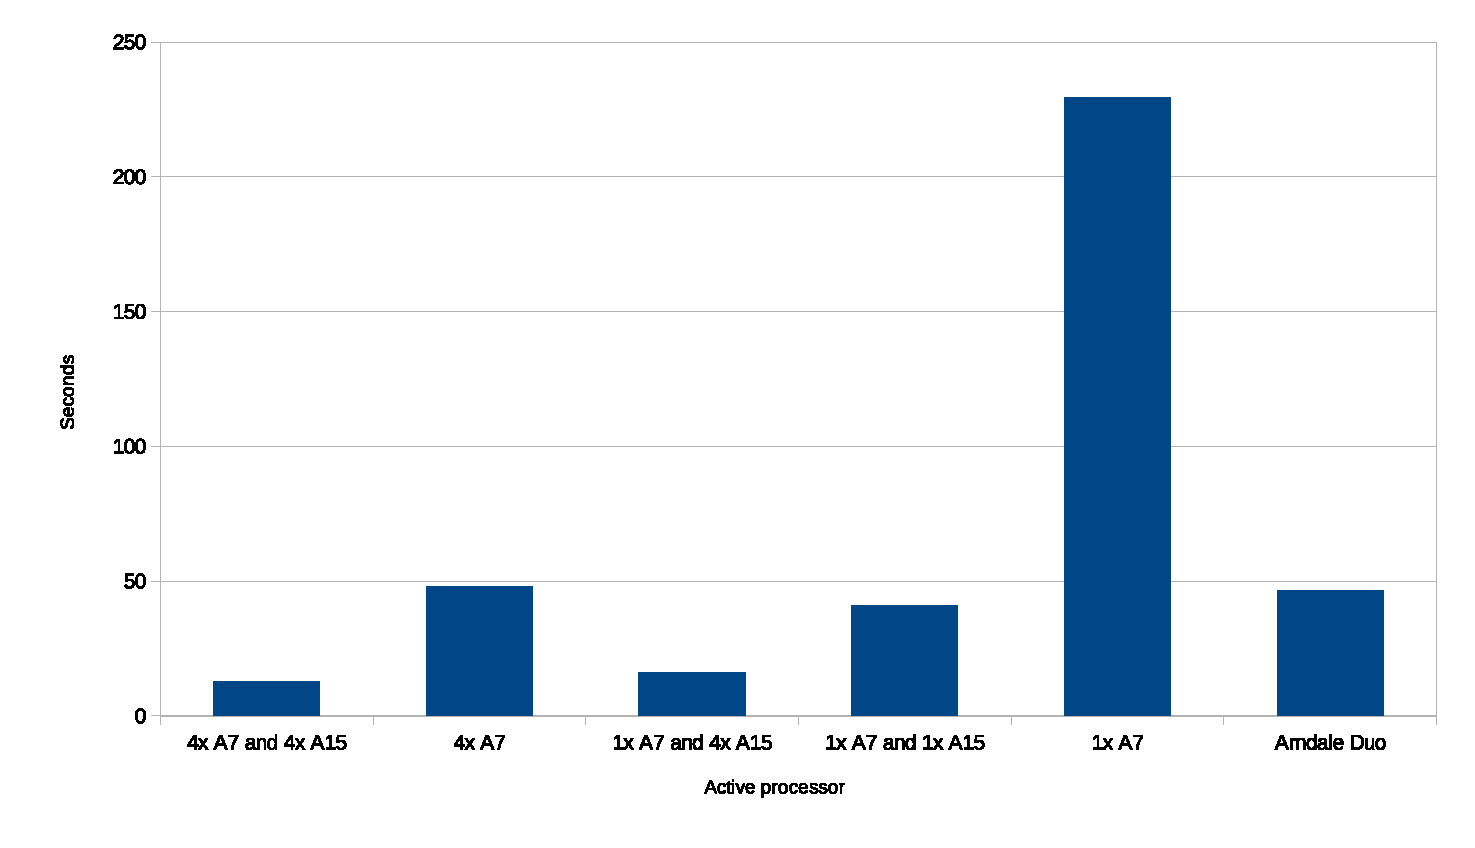
\includegraphics[width=160mm]{fig/execution-time-configurations.eps}
  \caption{Execution time of 2D-Convolution on different processor configurations. All results are from ODROID-XU3 were nothing is specified. The Arndale Duo is running at both it's ARM Cortex-A15 cores. The ARM Cortex-A15 cores of the ODROID-XU3 are running at 2.0 GHz, while they are running at 1.7 GHz on the Arndale Duo. \label{overflow}}
\end{figure}

\begin{figure}[H]
  \centering
  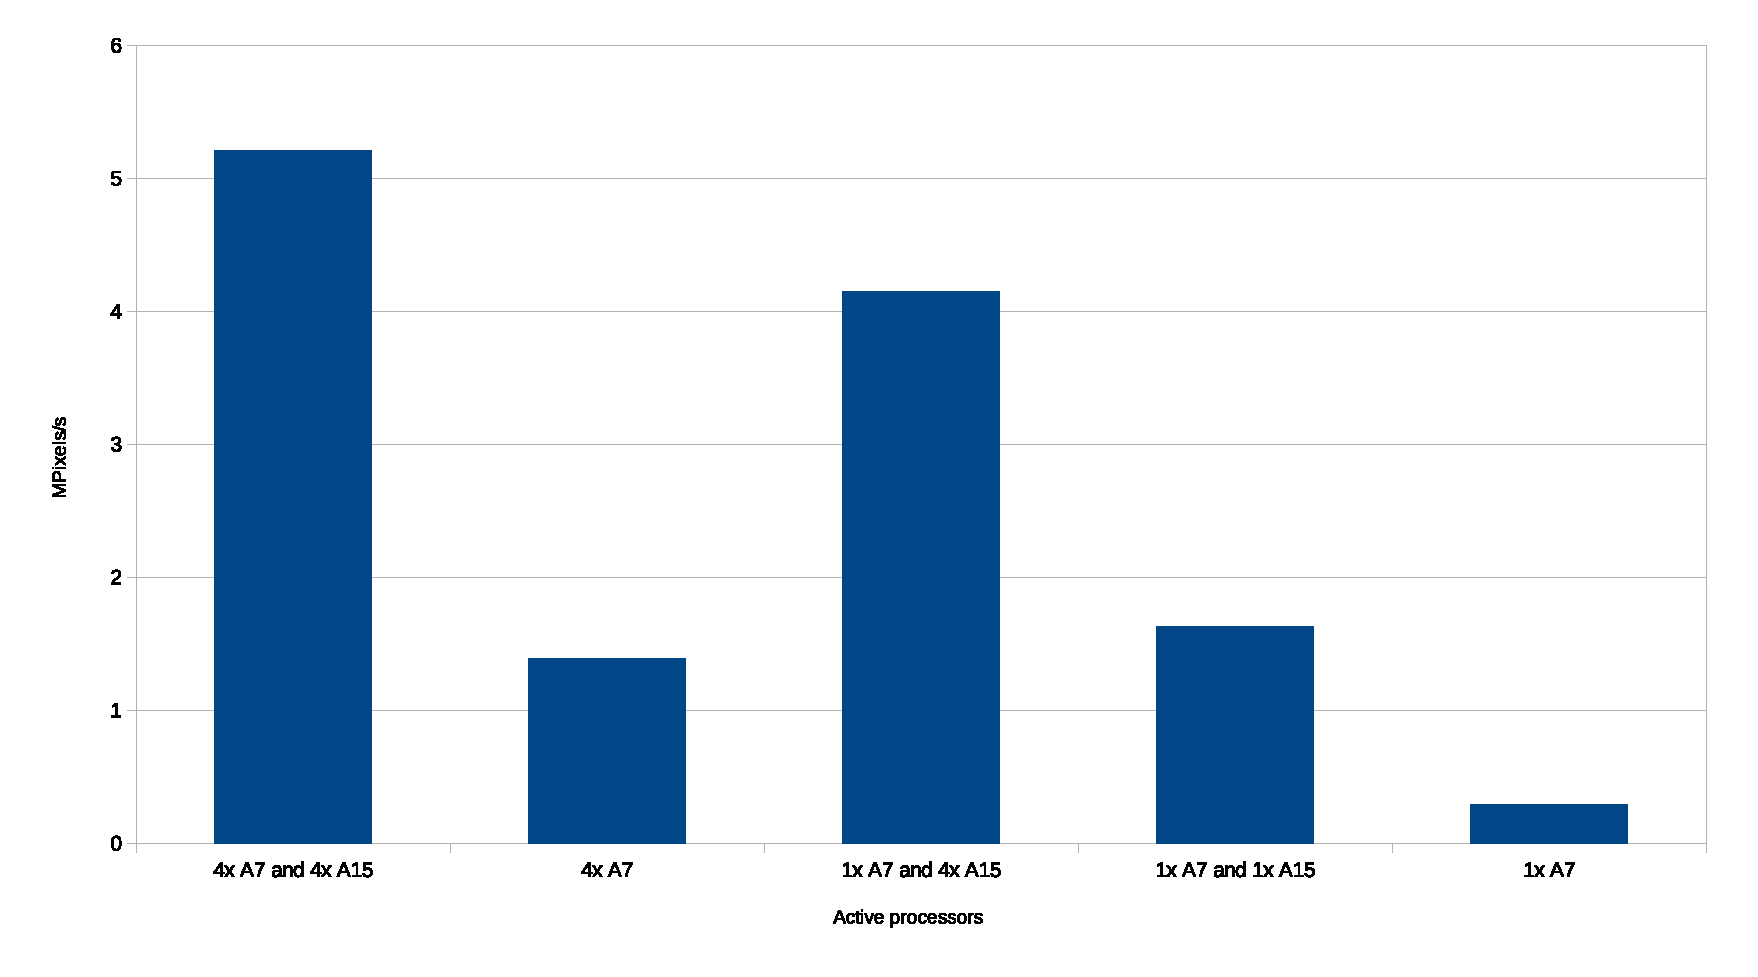
\includegraphics[width=160mm]{fig/mpixelss-configurations.eps}
  \caption{MPixels/s of 2D-Convolution running on different processor configurations. All results are from ODROID-XU3 were nothing is specified. The Arndale Duo is running at both it's ARM Cortex-A15 cores. The ARM Cortex-A15 cores of the ODROID-XU3 are running at 2.0 GHz, while they are running at 1.7 GHz on the Arndale Duo. \label{overflow}}
\end{figure}

\begin{table}[H]
  \begin{tabular}{llllll}
    \toprule
    Processor configuration           & Execution time (s)  & Performance (MPixels/s) \\
    \midrule
    4x Cortex-A7 and 4x Cortex-A15    & 12.8891             & 5.2066\\
    4x Cortex-A7                      & 48.1665             & 1.3932\\
    1x Cortex-A7 and 4x Cortex-A15    & 16.1658             & 4.1512\\
    1x Cortex-A7 and 1x Cortex-A15    & 41.1286             & 1.6316\\
    1x Cortex-A7                      & 229.3884            & 0.2925\\
    Arndale Duo with 2x Cortex-A15    & 46.3942             & 1.4465\\
    \bottomrule
  \end{tabular}
  \caption{Performance of 2D-Convolution with different processor configurations. All results are from ODROID-XU3 were nothing is specified. The ARM Cortex-A15 cores of the ODROID-XU3 are running at 2.0 GHz, while they are running at 1.7 GHz on the Arndale Duo. \label{overflow}}
\end{table}

As was to be expected, the large cores perform a lot better than the small ones.
Running the system with all 8 cores powered perform 3.7 times better than the small cores alone.
This is a large performance trade off, but the small cores are still useful if they have a low enough power consumption.

An interesting result here is that adding cores scale sub linearly.
The performance of 4 ARM Cortex-A7 cores and 4 ARM Cortex-A15 is only 3.19 times better than a single ARM Cortex-A7 and a single ARM Cortex-A15.
The reason behind this is likely to be related to memory congestion.
Even though 2D-Convolution is embarrassingly parallel, processor communication is not the only overhead with parallelization.
When running more processors, there are more processors to fight over the memory bandwidth and cause congestion.
This problem is likely to worsen with other more memory intensive problems, and problems with worse cache utilization.
This may lead to some situations where processor configurations, that does not perform well with 2D-Convolution, are well suited.
It would be interesting to explore this in the planned master thesis following this pilot project.

The performance of 4 ARM Cortex-A7 cores is 4.8 times better than a single ARM Cortex-A7.
The small cores seem to scale better than the large ones.
This may also be a result of the other tasks the operating system is running.
With less processing power available, the fraction of time spent running the operating system increase.
Because of this, there is reason to suspect that the small cores don't really scale as well as the results indicate.

The performance experiments run on the older Arndale Duo board show that it have worse performance with its ARM Cortex-A15 cores than the ODROID-XU3.
The two high power cores on the Arndale board have lower performance than a low power and a high power processor on the ODROID board.
If we assume linear scaling and extrapolate, we see that a quad core ARM Cortex-A15 with Arndale specifications would reach a performance of 2.9 MPixels/s.
On the ODROID-XU3, the similar setup with 4 ARM Cortex-A15 cores and an ARM Cortex-A7 core, had a performance of 4.2 MPixels/s.
The gap between the two is too large to be attributed to the single ARM Cortex-A7.
This performance difference is not surprising, as the Arndales cores run at a lower clock frequency.
They are also paired with slower memory, which may also contribute to the lower performance.

\section{Power measurements}
As described in chapter \fullref{setupandmethodology}, separate energy measurements for the different SoC components were gathered during execution of the experiments.
Each of the 4 components value was logged every 200 ms.
In figure \ref{powerovertime} you can see the raw energy measurements for a single execution of 2D-Convolution running on all 8 processors.
We can here observe the energy consumption of the program throughout the execution for different components.
The total energy consumption can be calculated from the data.
Observations regarding power usage during different execution stages can also be analyzed.
The same kind of data were gathered for a range of different processor configurations.

\begin{figure}[H]
  \centering
  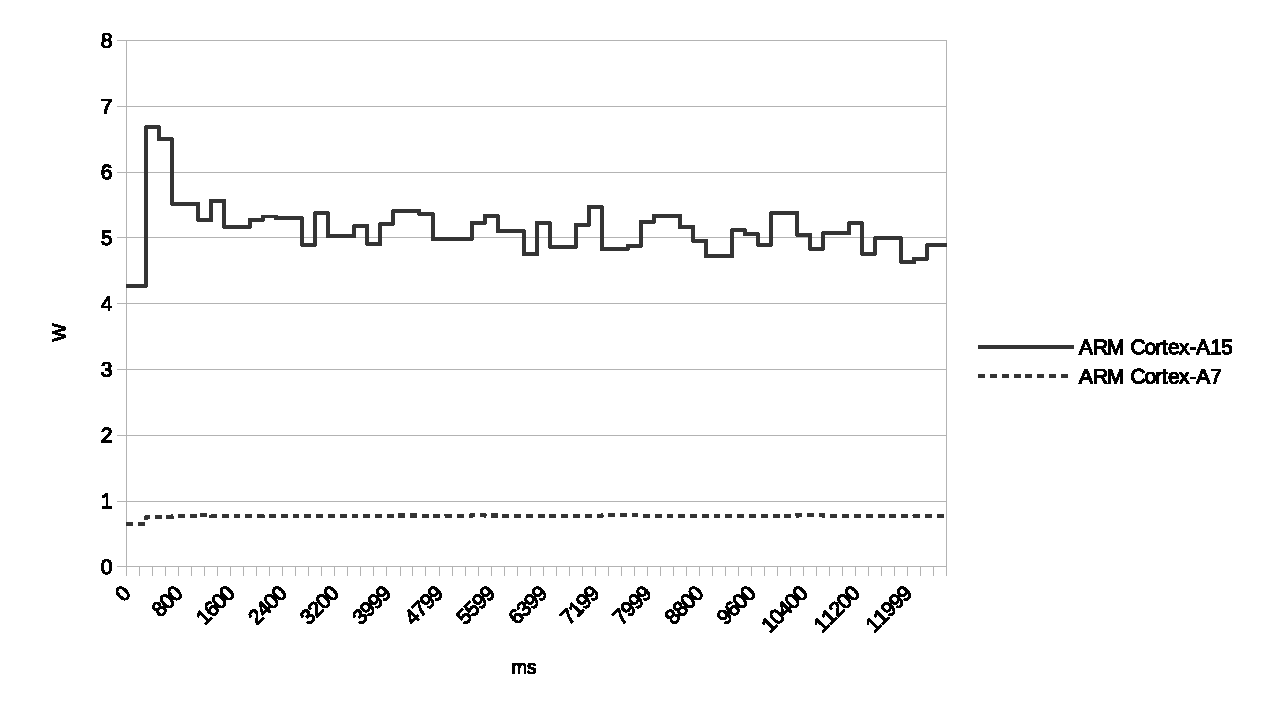
\includegraphics[width=160mm]{fig/power-over-time.eps}
  \caption{Power consumption for the large and small cores during execution of 2D-Convolution with unroll 8x. These results are from a full execution running on all 8 processors. \label{overflow}}\label{powerovertime}
\end{figure}
There is a spike in power consumption on both the small and large cores at the start of the execution.
This spike can be caused by a lot of different reasons.
There is not enough data to know what caused it.
Typical reasons for such spikes are intense operations during initiation of the program, or simply hardware implementations causing a power surge when processor cores are suddenly powered up from idle state.
For the rest of the execution there are variations in power consumption, but the consumption vary around the same general level.

\section{Average power measurements}
Using the data gathered for each component in different processor configurations we can examine their efficiency.
These data are presented in figure \ref{power-configurations}.
\begin{figure}[H]
  \centering
  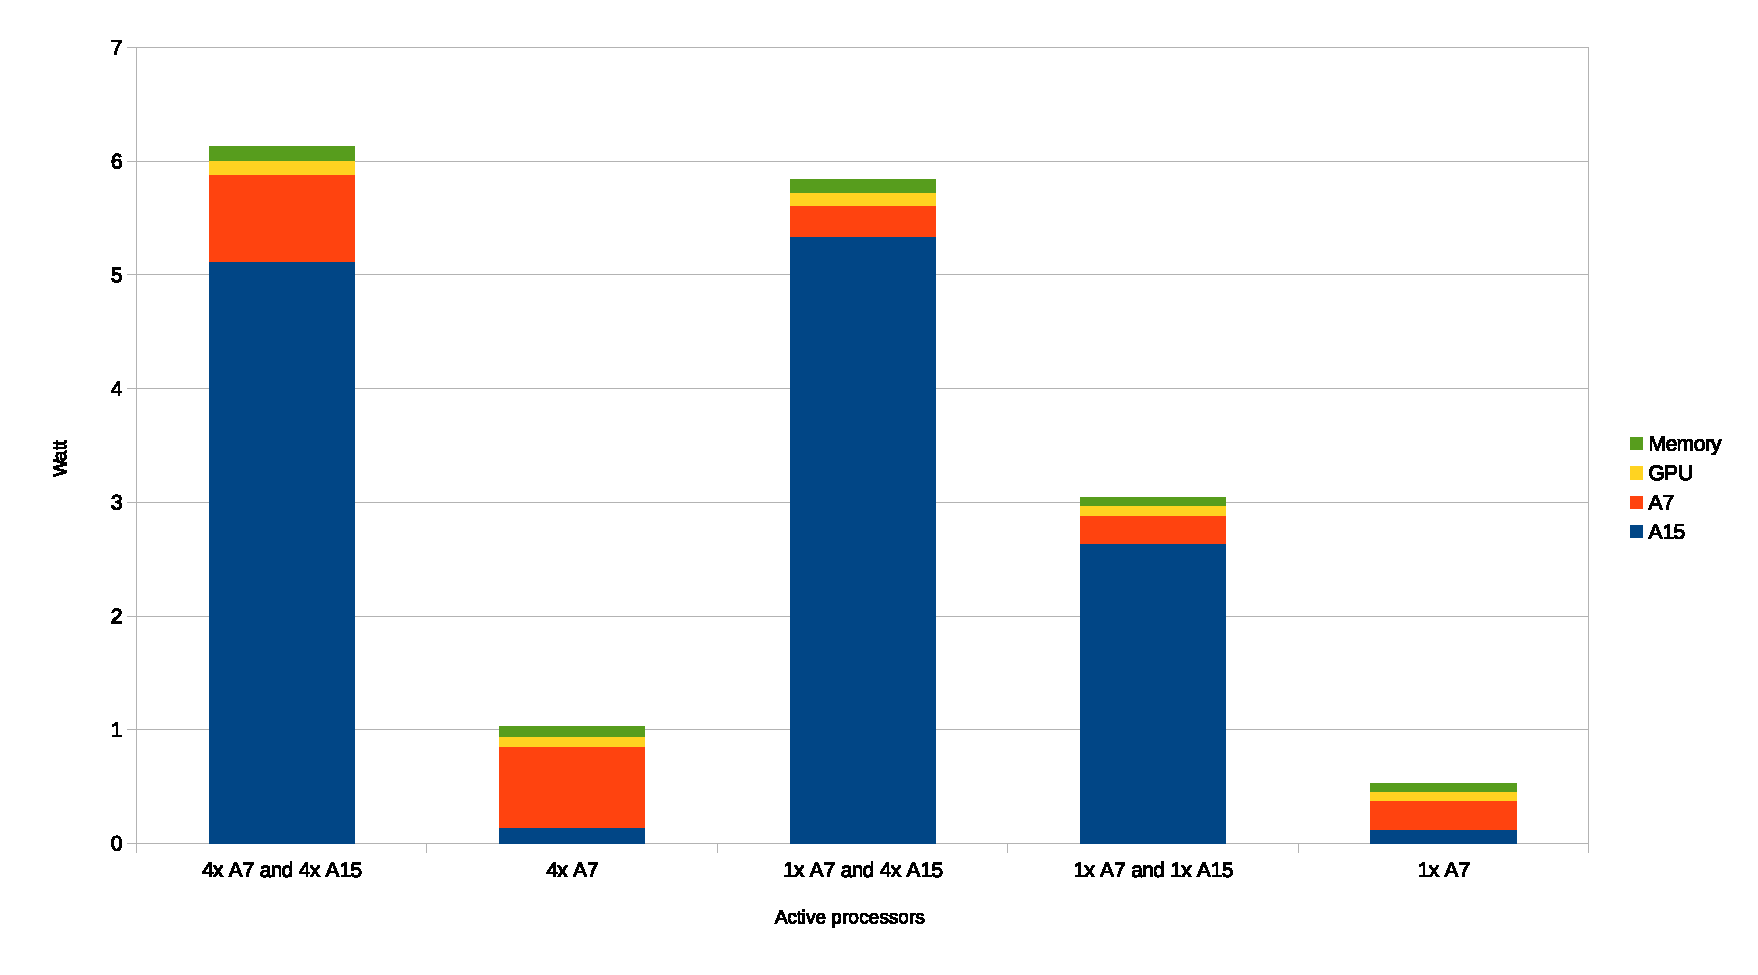
\includegraphics[width=160mm]{fig/power-configurations.eps}
  \caption{Average power consumed per second for different processors configurations running 2D-Convolution. The colors indicate different components, and the full height of each column is the accumulated total for the whole system.\label{overflow}} \label{power-configurations}
\end{figure}

\begin{table}[H]
  \begin{tabular}{llllll}
    \toprule
    Processor configuration         & \multicolumn{5}{c}{Power consumption per second for each component} \\
                                    & Cortex-A15  & Cortex-A7 & Mali-T628 & Memory  & Total \\
    \midrule
    4x Cortex-A7 and 4x Cortex-A15  & 5.1156          & 0.7693        & 0.1206        & 0.1208  & 6.1264 \\
    4x Cortex-A7                    & 0.1362          & 0.7157        & 0.0899        & 0.0817  & 1.0238 \\
    1x Cortex-A7 and 4x Cortex-A15  & 5.3356          & 0.2758        & 0.1161        & 0.1098  & 5.8373 \\
    1x Cortex-A7 and 1x Cortex-A15  & 2.6341          & 0.2540        & 0.0818        & 0.0755  & 3.0456 \\
    1x Cortex-A7                    & 0.1197          & 0.2535        & 0.0813        & 0.0709  & 0.5256 \\
    \bottomrule
  \end{tabular}
  \caption{Execution time of 2D-Convolution with different degrees of loop unrolling on different processor configurations. \label{overflow}}
\end{table}

As expected we see that the power of the ARM Cortex-A7s is a lot lower than the power of the ARM Cortex-A15.
Turning off the power hungry Cortex-A15s reduce the total power to a sixth (0.17).
This is useful for applications running that do not require high performance, and  want to consume low power.
This way of power saving can be increased even more by utilizing only a single Cortex-A7.
This configuration is have the lowest power consumption per second, and is useful for standing by, or executing minor calculations while standing by.
Running on only a single Cortex-A7 reduce the power of the system to a tenth (0.10) of that of the fully powered 8 core system.
More than half of this power was used by other components.

In addition to the total power of the system, the results also allow us to analyze the power of each component.
Turning off 3 Cortex-A15 cores only reduce the power to about half (0.51).
Even turning all the Cortex-A15 cores off still leave some power consumed by them.
Because of this power, running the system with only four Cortex-A7 cores still spend 13\% of the total energy on the Cortex-A15 cores, which are not doing any work.
Similarly turning off 3 Cortex-A7 cores only reduce power to a bit more than two thirds (0.35).
These results reveal that the energy for each set of cores are not spent solely on powering the cores themselves, but also some peripheral components related to the cores.
These peripheral components can not be turned partially of, and will consume some power when at least one core is on.
They even consume some power when the cores are all off.
Because of this overhead power from partially powered processors, there rarely occur situations where this is optimal.
The results for such processor configurations will be analyzed further in this thesis to observe whether or not this is the case here.
\section{Energy consumption measurements}A \label{energyconsumptionmeasurements}
The power usage of the different system components is interesting.
There is however many cases where the system can be put to another task, or shut down, when it is finished.
In such cases it is interesting to observe the total amount of energy consumed completing the task.
In figure \ref{power-consumed-configurations} the data for each component power usage is multiplied with the execution time.
The data height of each column is the amount of energy consumed.

\begin{figure}[H]
  \centering
  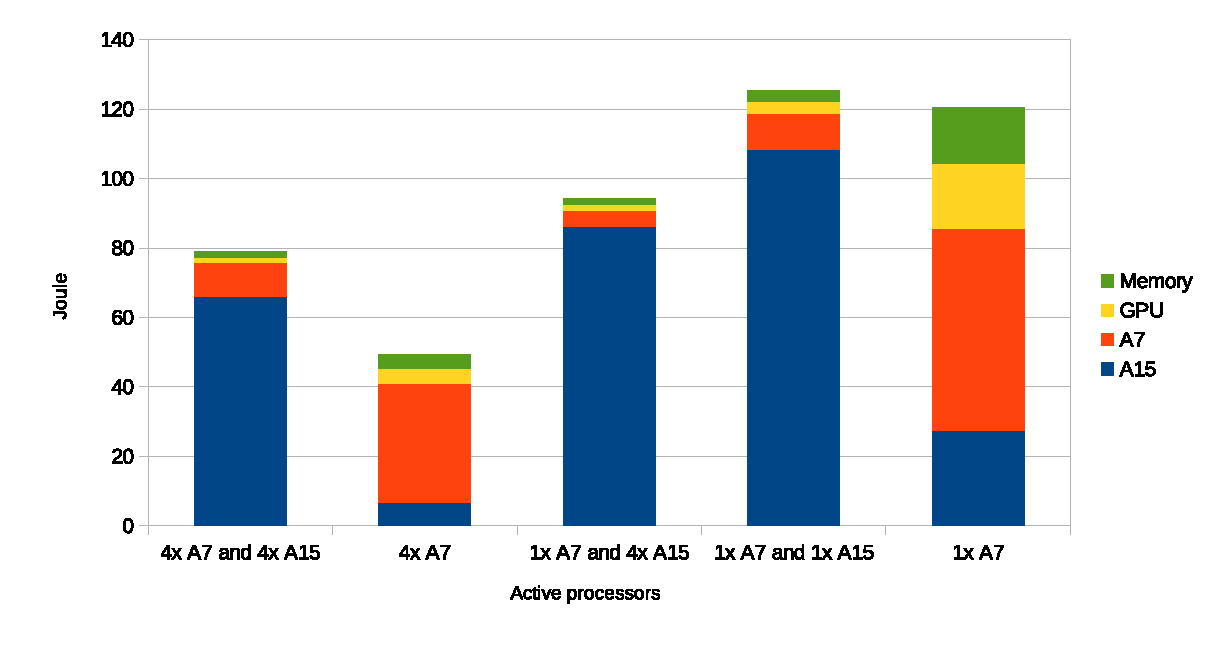
\includegraphics[width=160mm]{fig/power-consumed-configurations.eps}
  \caption{Total energy consumption execution the whole 2D-Convolution program. The colors indicate different components, and the full height of each column is the accumulated total power consumed for the whole system.\label{overflow}} \label {power-consumed-configurations}
\end{figure}

Figure \ref{power-consumed-configurations} show that, even though the fully powered system with all eight processors operating performed better than all the other processor configurations, it is not the best at energy consumption.
The power consumed by a full execution of 2D-Convolution on all 8 processors consume 60\% more power than running it on the 4 Cortex-A7 cores alone.
Running on the more energy efficient, processors cost performance, but it save energy.
This is a trade off that is often observed in energy efficiency.
It vary from application to application what is the preferred property, but it is always an issue of balancing the two.
In section \fullref{EDP} the balance point between performance and energy of these experiments are explored in further depth.

Apart from the results for the full eight core system and the 4 small cores, experiments for the other processor configurations were also carried out.
These results however, were not promising.
All the other processor configurations had higher energy consumption than the two first configurations.
They their performance was also worse than the full system, which completed the execution with a lower power consumption.
In other words, they did neither stand out in energy efficiency or performance.
There may exist potential situations with very specific maximum execution times and such, where these configurations may be viable.
They are however not promising candidates for general applications.

\section{Energy Delay Product (EDP) measurements} \label{EDP}
While the energy consumption is a good energy measure in many situations, it is often interesting to compare the energy consumed with it's performance trade off.
As explained in section \fullref{energymeasurement} energy delay product measurements can be used to examine this trade off.
These are the energy data from chapter \ref{energyconsumptionmeasurements} multiplied with the execution time of the respective application execution.

\begin{figure}[H]
  \centering
  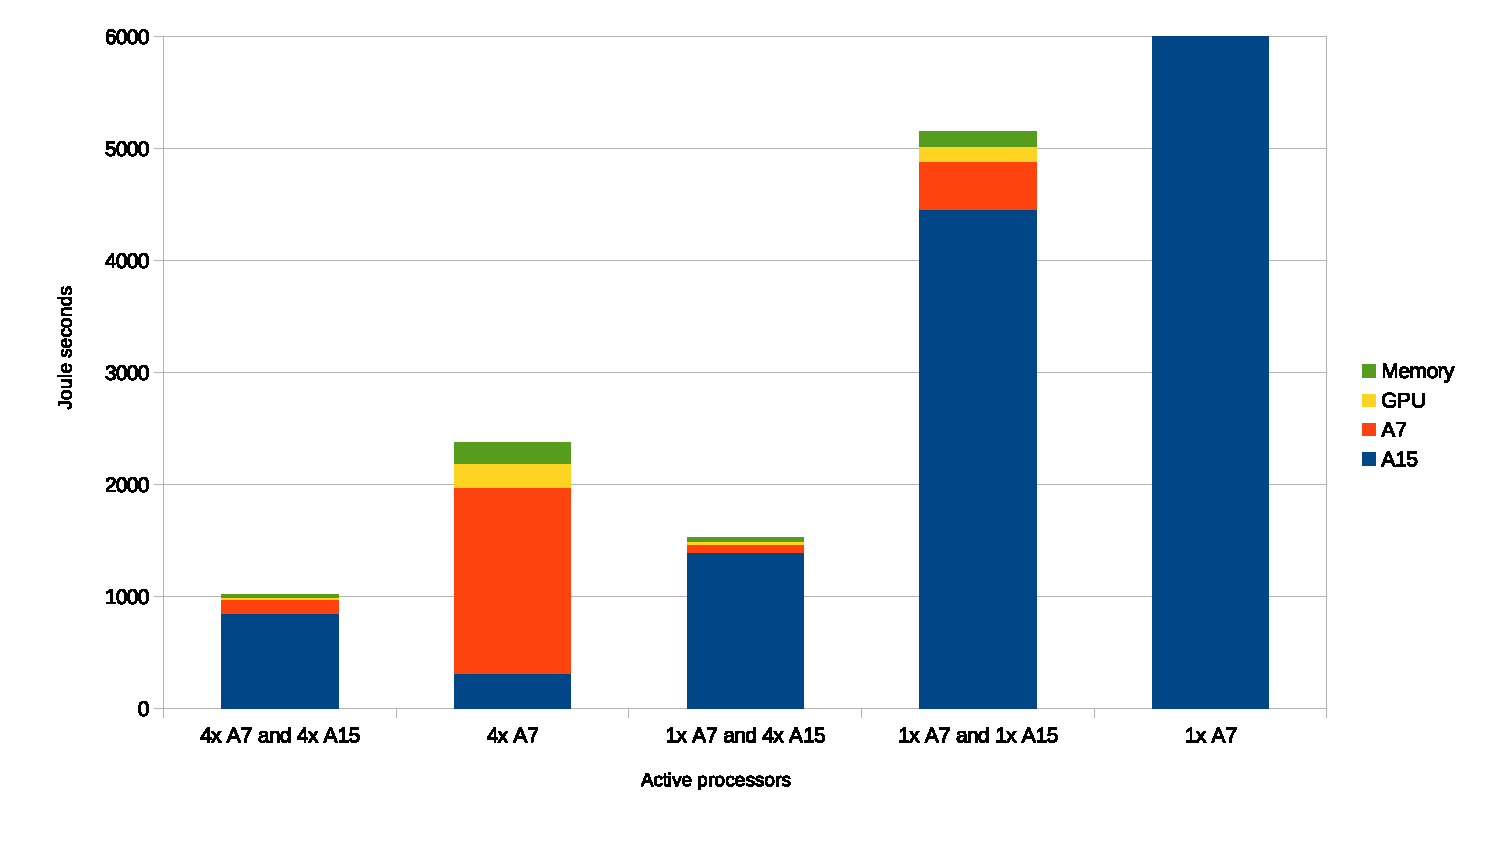
\includegraphics[width=160mm]{fig/EDP-configurations.eps}
  \caption{Energy delay product after execution the whole 2D-Convolution program with different processor configurations. Note that the EDP of the ARM Cortex-A7 goes beyond the scale of the graph with a value of 27658, to allow for better readability. The colors indicate different components, and the full height of each column is the accumulated energy delay product for the whole system.\label{overflow}} \label {EDP-configurations}
\end{figure}

These data clearly show that with energy delay product as out goal, running the fully powered system achieve the best results.
The energy efficiency gain by switching to the smaller and more energy efficient processors, is not worth the performance trade off.
This mean that for applications which require a balanced performance trade off, the more energy efficient Cortex-A7 cores will not be a great alternative in most cases.

It is worth noting that the configuration running on only 1 of the small cores and all the large ones have a decent EDP.
There may exist special cases where this processor configuration may be useful.
It is also obvious that running on the single Cortex-A7 processor, while having the lowest power measurement, is unsuited for any application with performance demand.

